\documentclass{beamer}
\usepackage[utf8]{inputenc}

\usetheme{Madrid}
\usecolortheme{default}
\usepackage{amsmath,amssymb,amsfonts,amsthm}
\usepackage{txfonts}
\usepackage{multicol}
\usepackage{tkz-euclide}
\usepackage{listings}
\usepackage{adjustbox}
\usepackage{array}
\usepackage{tabularx}
\usepackage{gvv}
\usepackage{lmodern}
\usepackage{circuitikz}
\usepackage{tikz}
\usepackage{graphicx}
\usepackage{hyperref}

\setbeamertemplate{page number in head/foot}[totalframenumber]

\usepackage{tcolorbox}
\tcbuselibrary{minted,breakable,xparse,skins}



\definecolor{bg}{gray}{0.95}
\DeclareTCBListing{mintedbox}{O{}m!O{}}{%
  breakable=true,
  listing engine=minted,
  listing only,
  minted language=#2,
  minted style=default,
  minted options={%
    linenos,
    gobble=0,
    breaklines=true,
    breakafter=,,
    fontsize=\small,
    numbersep=8pt,
    #1},
  boxsep=0pt,
  left skip=0pt,
  right skip=0pt,
  left=25pt,
  right=0pt,
  top=3pt,
  bottom=3pt,
  arc=5pt,
  leftrule=0pt,
  rightrule=0pt,
  bottomrule=2pt,
  toprule=2pt,
  colback=bg,
  colframe=orange!70,
  enhanced,
  overlay={%
    \begin{tcbclipinterior}
    \fill[orange!20!white] (frame.south west) rectangle ([xshift=20pt]frame.north west);
    \end{tcbclipinterior}},
  #3,
}
\lstset{
    language=C,
    basicstyle=\ttfamily\small,
    keywordstyle=\color{blue},
    stringstyle=\color{orange},
    commentstyle=\color{green!60!black},
    numbers=left,
    numberstyle=\tiny\color{gray},
    breaklines=true,
    showstringspaces=false,
}
%------------------------------------------------------------
%This block of code defines the information to appear in the
%Title page
\title %optional
{4.13.9}
\date{September 20,2025}
%\subtitle{A short story}

\author % (optional)
{Aditya Appana - EE25BTECH11004}



\begin{document}


\frame{\titlepage}
\begin{frame}{Question}
Let the algebraic sum of the perpendicular distances from the points (2,0),(0,2) and
(1,1) to a variable straight line be zero; then the line passes through a fixed point
whose coordinates are \rule{1.5cm}{0.15mm}.
\end{frame}



\begin{frame}[fragile]
    \frametitle{Formulae}
The normal form of a line is:
\begin{align}
\vec{n}^Tx = c
\end{align}\\
The perpendicular distance of a point from a line is:
\begin{align}
\frac{|\vec{n}^Tx - c|}{||n||}
\end{align}\\

\end{frame}

\begin{frame}[fragile]
    \frametitle{Solution}
It is given that the algebraic sum of the perpendicular distances of three points (2,0), (0,2), and (1,1) to a line $\vec{n}^Tx = c$ is 0. Therefore:

\begin{align}
\frac{\vec{n}^Tx_1 - c}{||n||} + \frac{\vec{n}^Tx_2 - c}{||n||} + \frac{\vec{n}^Tx_3 - c}{||n||} = 0
\end{align}\\
\end{frame}

\begin{frame}[fragile]
\frametitle{Solution}
\begin{align}
\frac{\vec{n}^T(\vec{x}_1 +\vec{x}_2+ \vec{x}_3)- 3c}{||n||} = 0
\end{align}
So, the required point is:

\begin{align}
\frac{(\vec{x}_1 +\vec{x}_2+ \vec{x}_3)}{3}
\end{align}

Substituting the points:
\begin{align}
\frac{\myvec{2\\0} + \myvec{0\\2} + \myvec{1\\1} }{3} =\\
\myvec{1\\1}
\end{align}\\
Therefore the line passes through the fixed point (1,1).
\end{frame}

\begin{frame}[fragile]
\frametitle{Python Code}
\begin{lstlisting}
import numpy as np
import matplotlib.pyplot as plt

fig = plt.figure(figsize = (6,6))
ax = fig.add_subplot(111)
ax.set_aspect('equal', adjustable='box')
ax.set_title("Three Points")

vector = str(input("Input the vectors, and input X when you are done"))

counter = 0;
sum = np.zeros(2)
\end{lstlisting}
\end{frame}
\begin{frame}[fragile]
\frametitle{Python Code}
\begin{lstlisting}

while(vector != "X"):
    vector.strip()
    vector0, vector1 = vector.split(" ")
    vector0 = int(vector0)
    vector1= int(vector1)
    vectorA = np.array([vector0,vector1])
    sum += vectorA
    counter = counter + 1
    ax.scatter(vector0, vector1, label = f'({vector0}, {vector1})')
    vector = str(input("Input the next vector"))
    
commonpoint = sum/counter
print(f"The line passes through ( {commonpoint[0]}, {commonpoint[1]} )")
plt.legend()
ax.grid(True)
plt.show()


\end{lstlisting}
\end{frame}

\begin{frame}[fragile]
\frametitle{Python Code}


\begin{figure}[H]
    \centering
    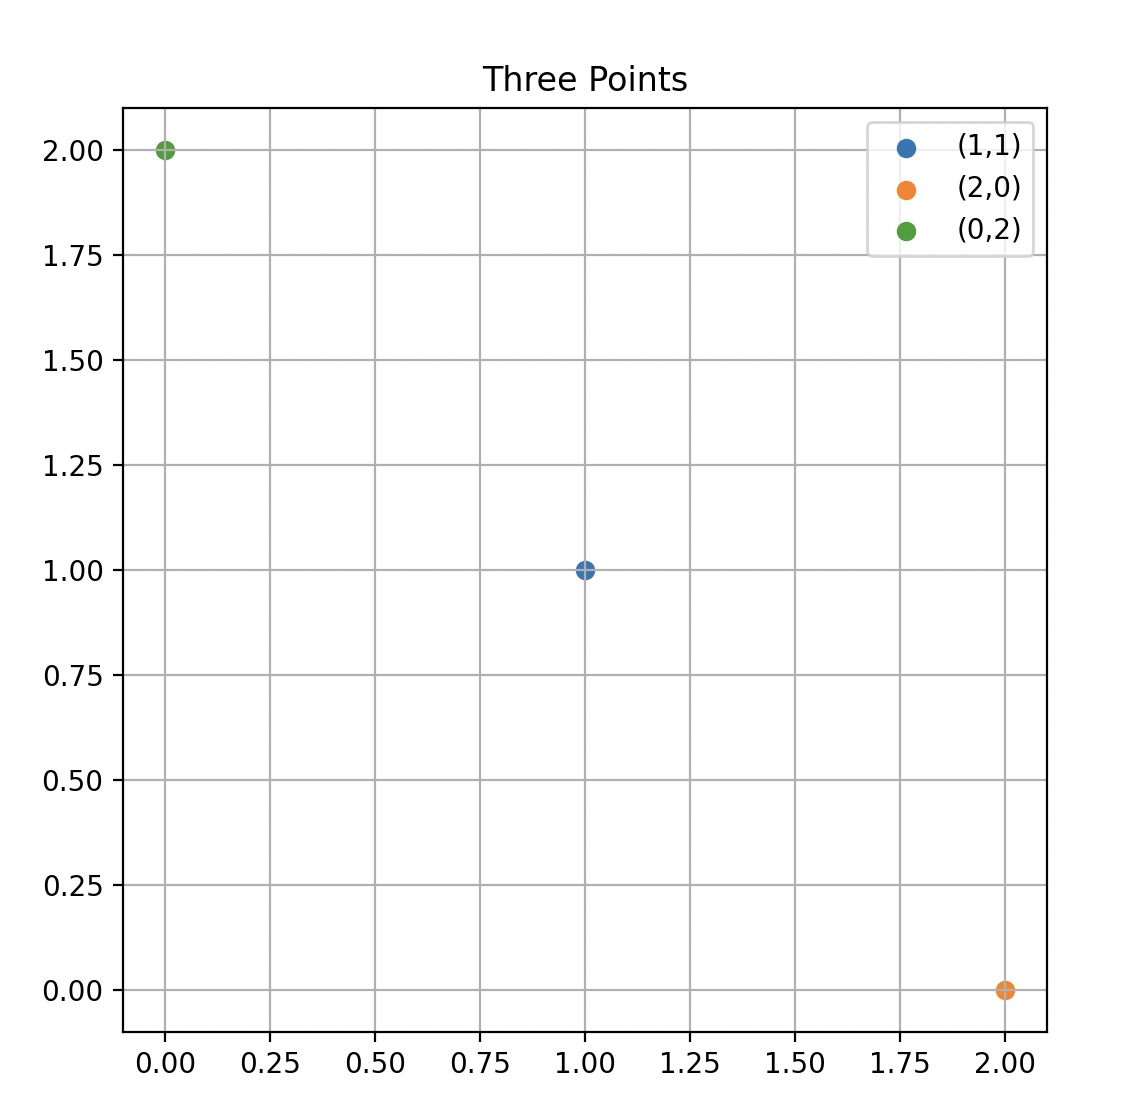
\includegraphics[width=0.7\columnwidth]{Figs/527.png}
    \caption{Plot}
    \label{fig:placeholder}
\end{figure} 

\end{frame}

\end{document}